\chapter{RESULTS}

\section{User \& Account Creation}

The platform follows a unique approach where each server is dedicated to a single user. However, within that server, the user can create and manage multiple accounts. This setup ensures full ownership and control over data while still enabling interaction within the federated network.

\subsection{User Creation}
To set up a user, the individual must provide a valid email address and set a secure password. This step ensures authentication and account recovery options. Once the user is registered, they gain full control over their server and can proceed to create multiple accounts as needed.

\begin{figure}[h!]
    \centering
    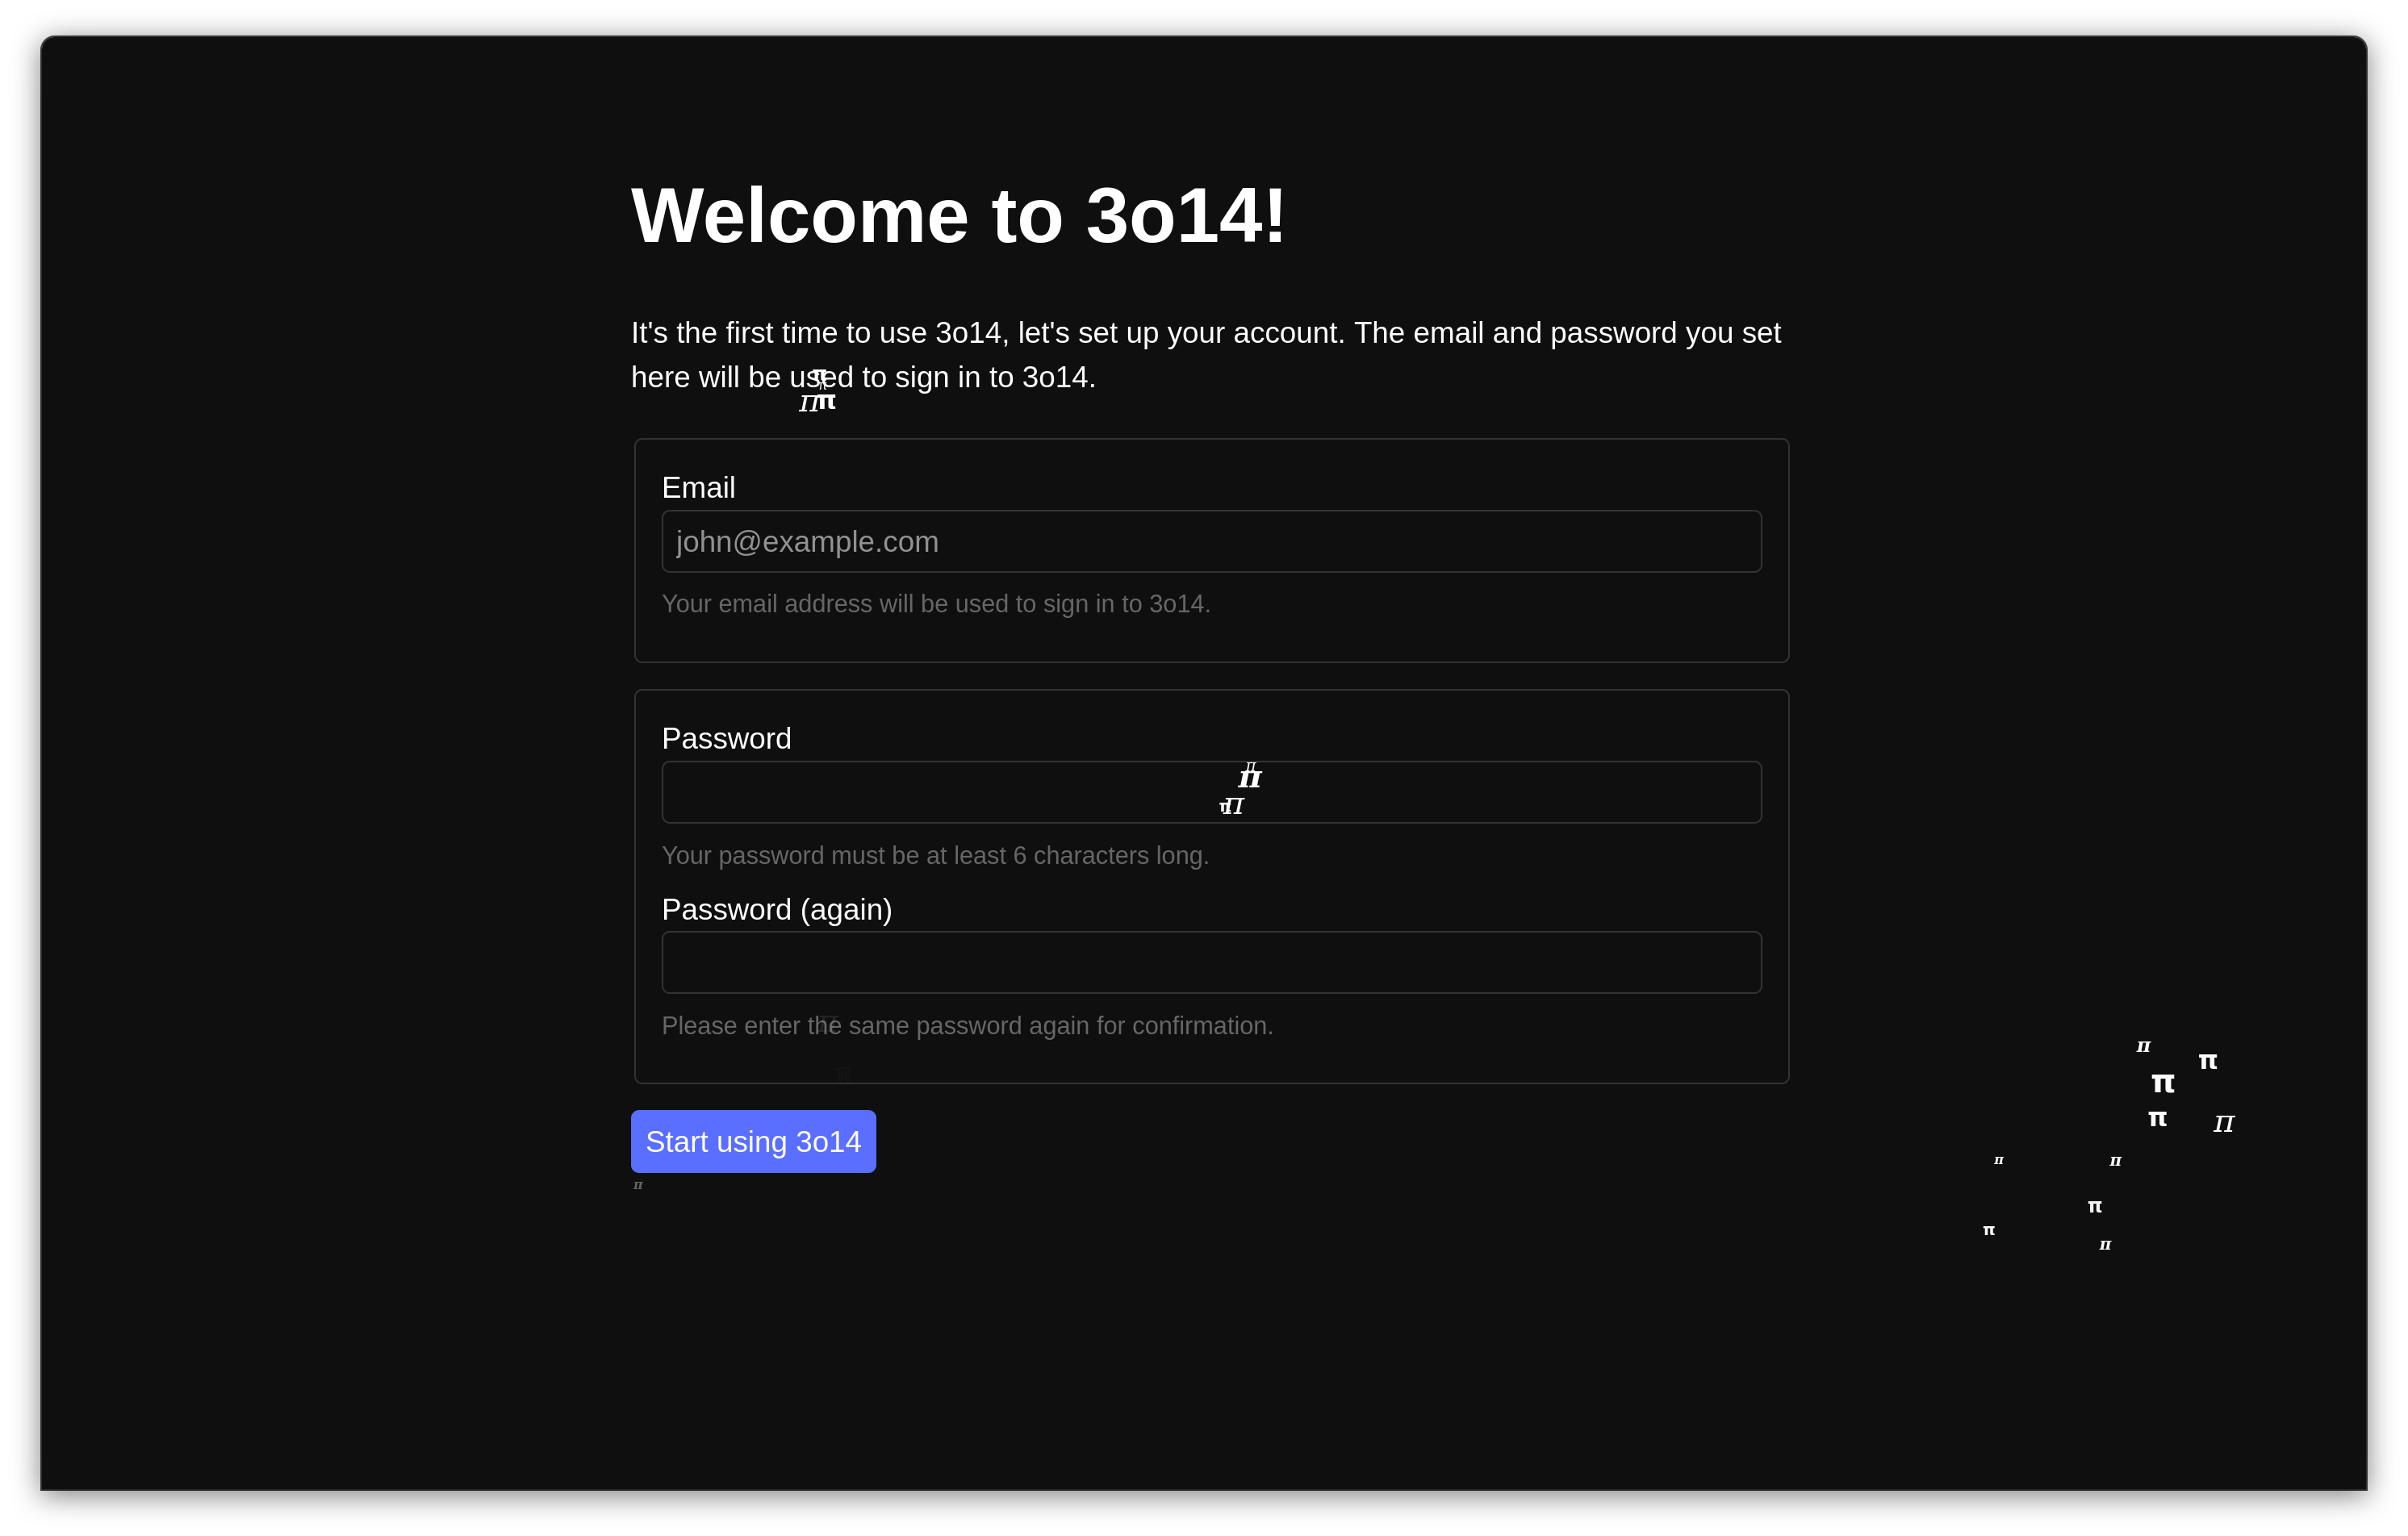
\includegraphics[width=0.5\textwidth]{Graphics/usercreation.png}
    \caption{User Creation}
    \label{fig:user_creation}
\end{figure}

\subsection{Account Creation}
Within their personal server, the user can create and manage multiple accounts. Each account can have distinct identities, preferences, and privacy settings while still operating under the same server. This feature allows for flexibility in communication, enabling users to maintain separate professional and personal identities, for example.

\begin{figure}[h!]
    \centering
    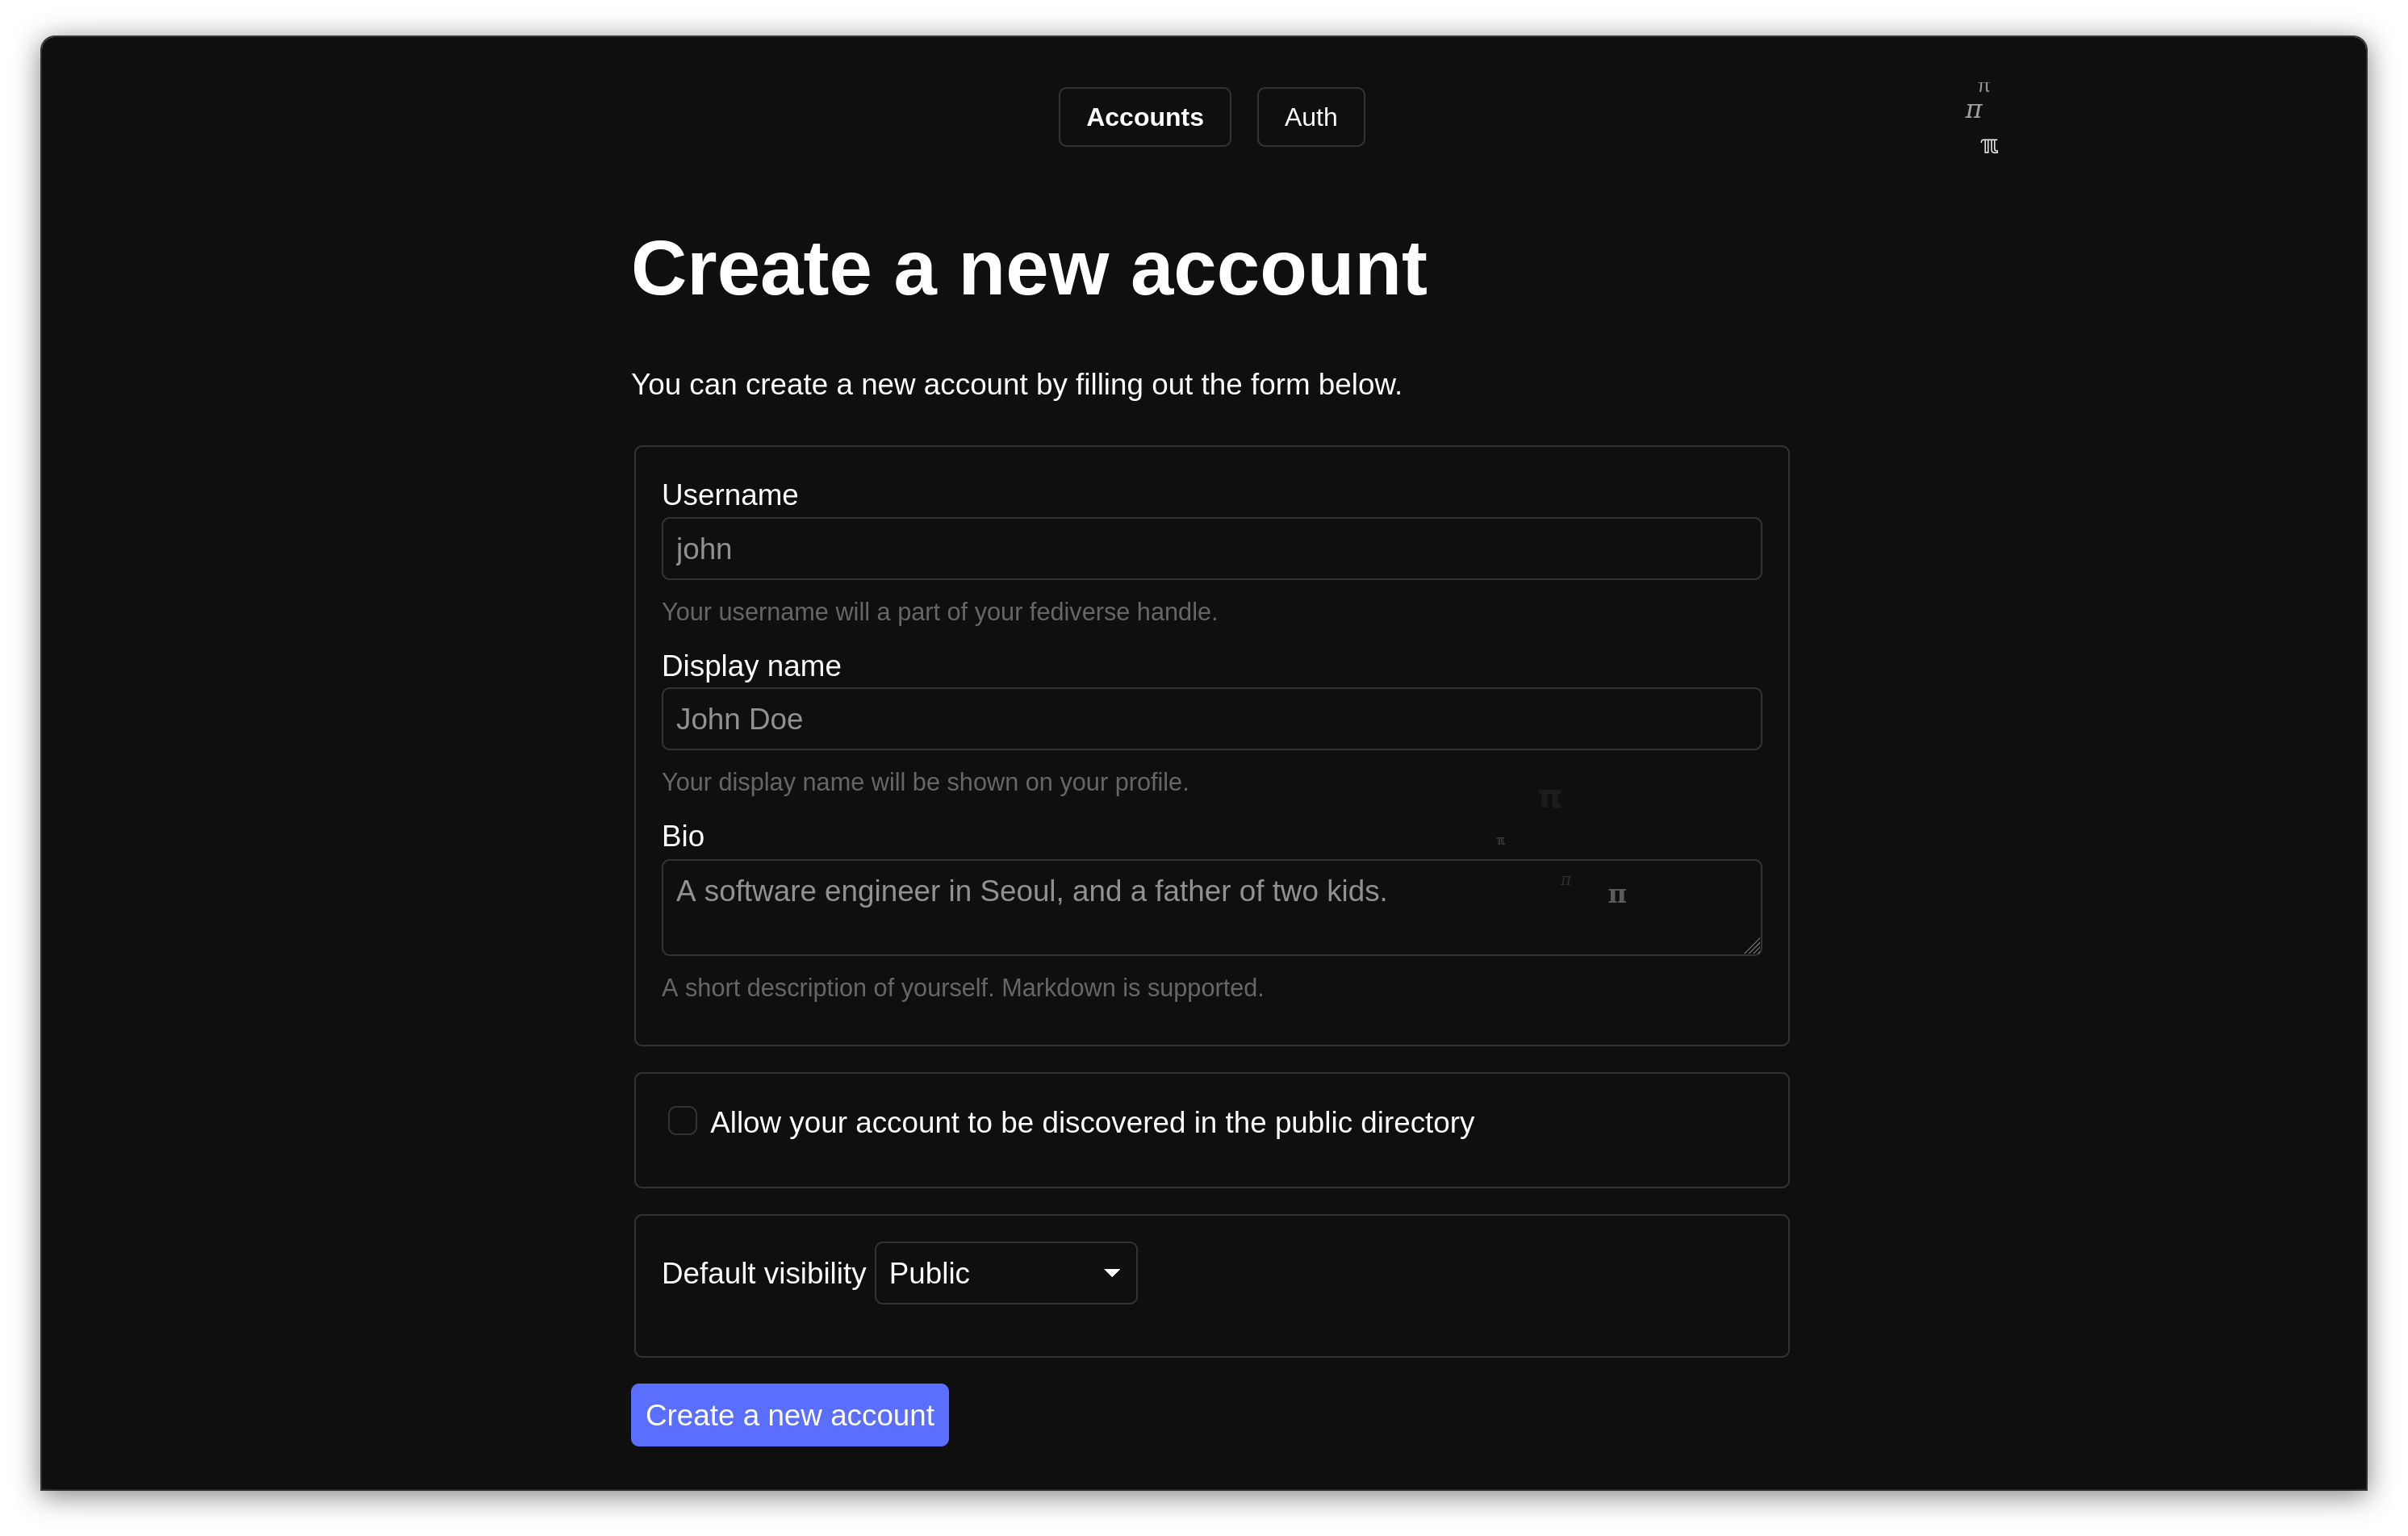
\includegraphics[width=0.5\textwidth]{Graphics/accountcreation.png}
    \caption{Account Creation}
    \label{fig:account_creation}
\end{figure}

\section{Posting Status With Latex}

Users can include mathematical expressions within plaintext using LaTeX syntax while composing a post. As shown in Figure~\ref{fig:writing_post}, the application provides a live preview of the rendered LaTeX output, allowing users to verify their equations before posting. Once published, the post is displayed in the timeline with properly formatted LaTeX expressions, as demonstrated in Figure~\ref{fig:post_in_timeline}. This feature ensures that complex mathematical notations, scientific formulas, and equations are easily readable and visually appealing in posts.

\begin{figure}[htbp]
  \centering
  % First image in its own minipage
  \begin{minipage}[b]{0.45\linewidth}
    \centering
    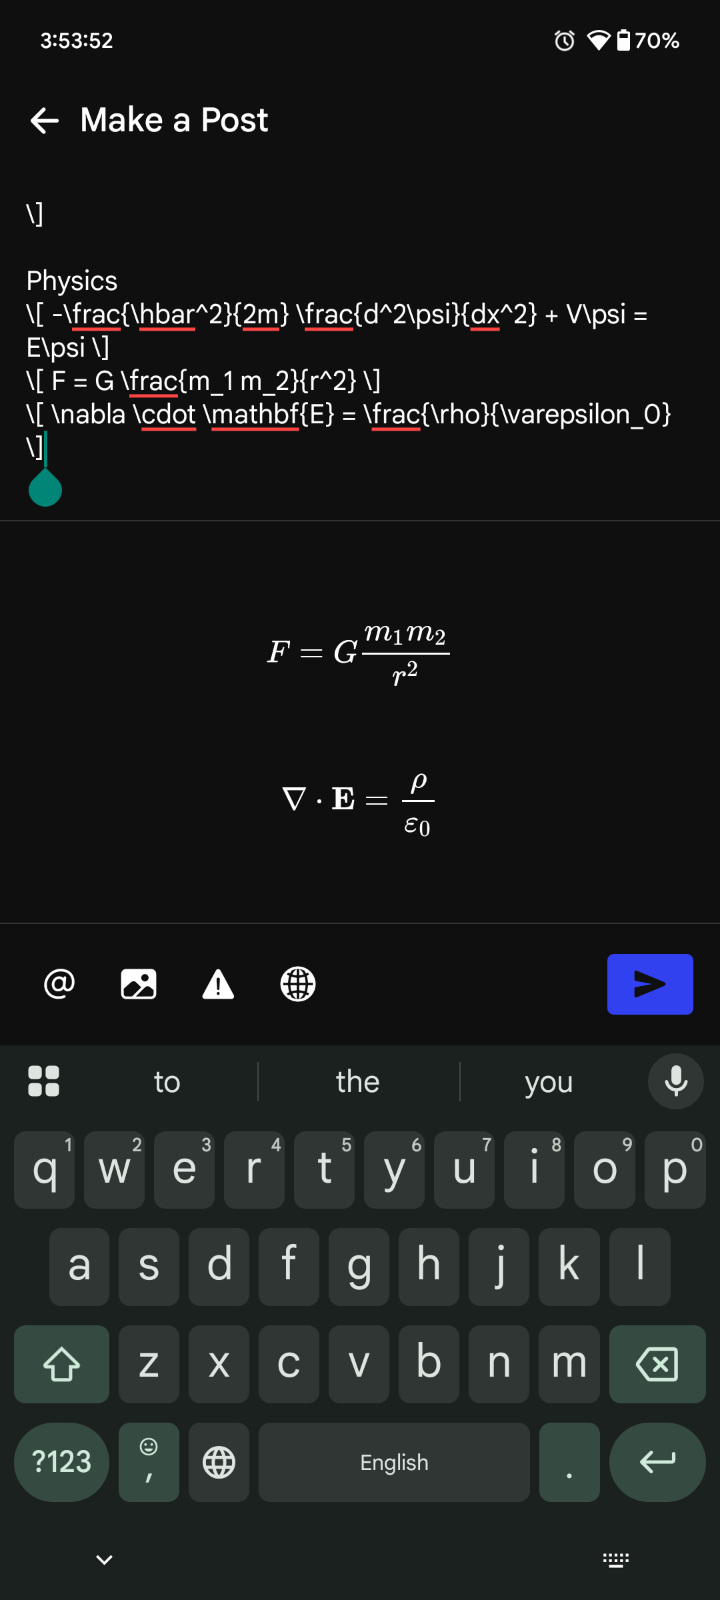
\includegraphics[width=\linewidth]{Graphics/writingpost.png}
    \caption{Live rendering of latex while writing post}
    \label{fig:writing_post}
  \end{minipage}
  \hfill % adds some space between images
  % Second image in its own minipage
  \begin{minipage}[b]{0.45\linewidth}
    \centering
    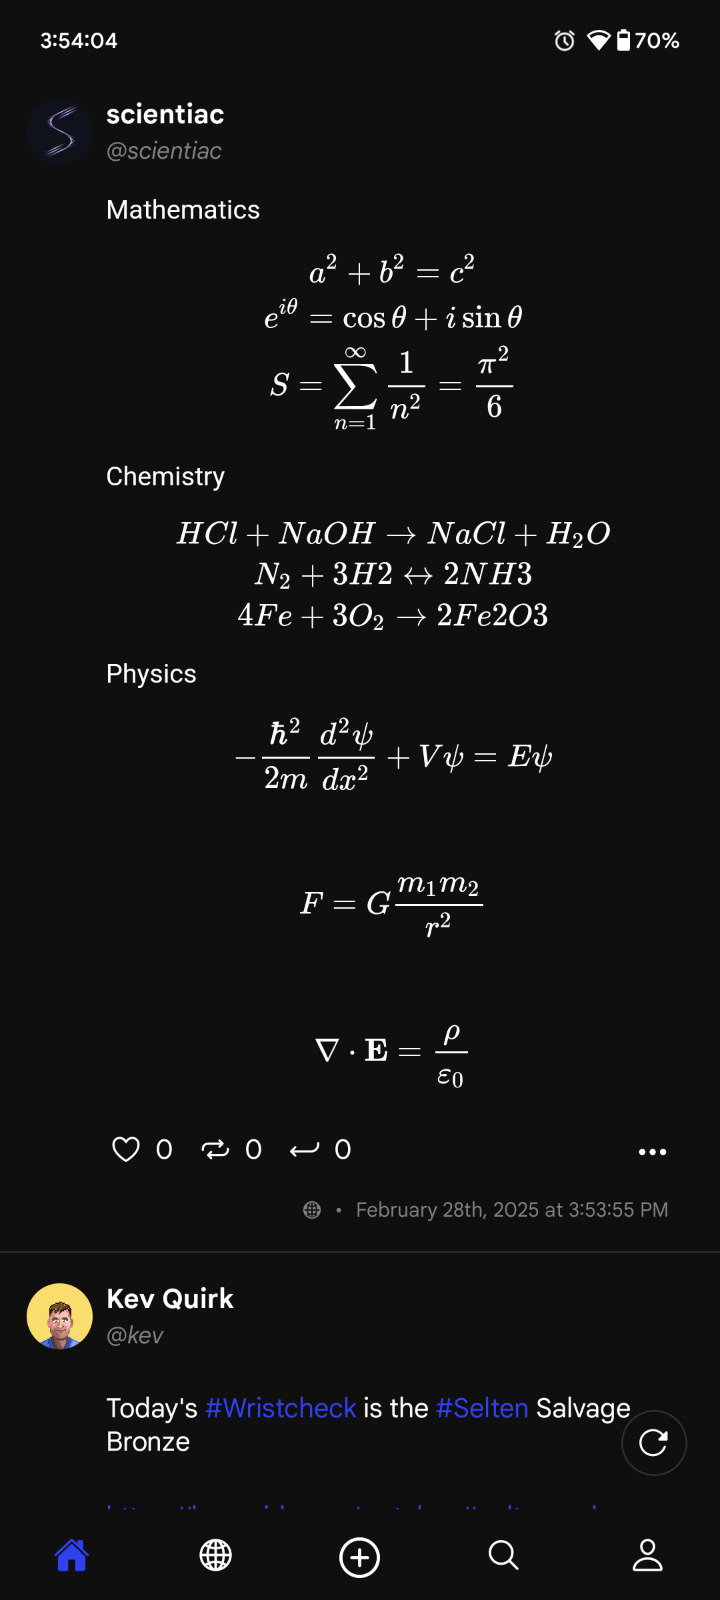
\includegraphics[width=\linewidth]{Graphics/postintimeline.png}
    \caption{Rendered post with latex in timeline}
    \label{fig:post_in_timeline}
  \end{minipage}
\end{figure}

\clearpage

\section{Interaction with Remote Accounts}
User, using their account, can interact with other users on different instances or services using ActivityPub\cite{ActivityPub} constructs like Follow, Like, Boost, Reply. 

\subsection{Searching and Following Remote Accounts}
Users can search for remote accounts by entering the handle associated with an account on a different instance. As shown in Figure~\ref{fig:search_follow}, the search results display matching accounts along with relevant details, allowing users to identify and interact with the desired profile.

Once a remote account is found, users can visit its profile page (Figure~\ref{fig:remote_profile}), where they can view posts, follow the account, and engage through actions like liking or boosting posts. This seamless integration enables cross-instance communication within the network.
\begin{figure}[htbp]
  \centering
  % First image in its own minipage
  \begin{minipage}[b]{0.45\linewidth}
    \centering
    
\includegraphics[width=\linewidth]{Graphics/remoteaccountsearchfollow.png}
    \caption{Searching and following remote accounts}
    \label{fig:search_follow}
  \end{minipage}
  \hfill % adds some space between images
  % Second image in its own minipage
  \begin{minipage}[b]{0.45\linewidth}
    \centering
    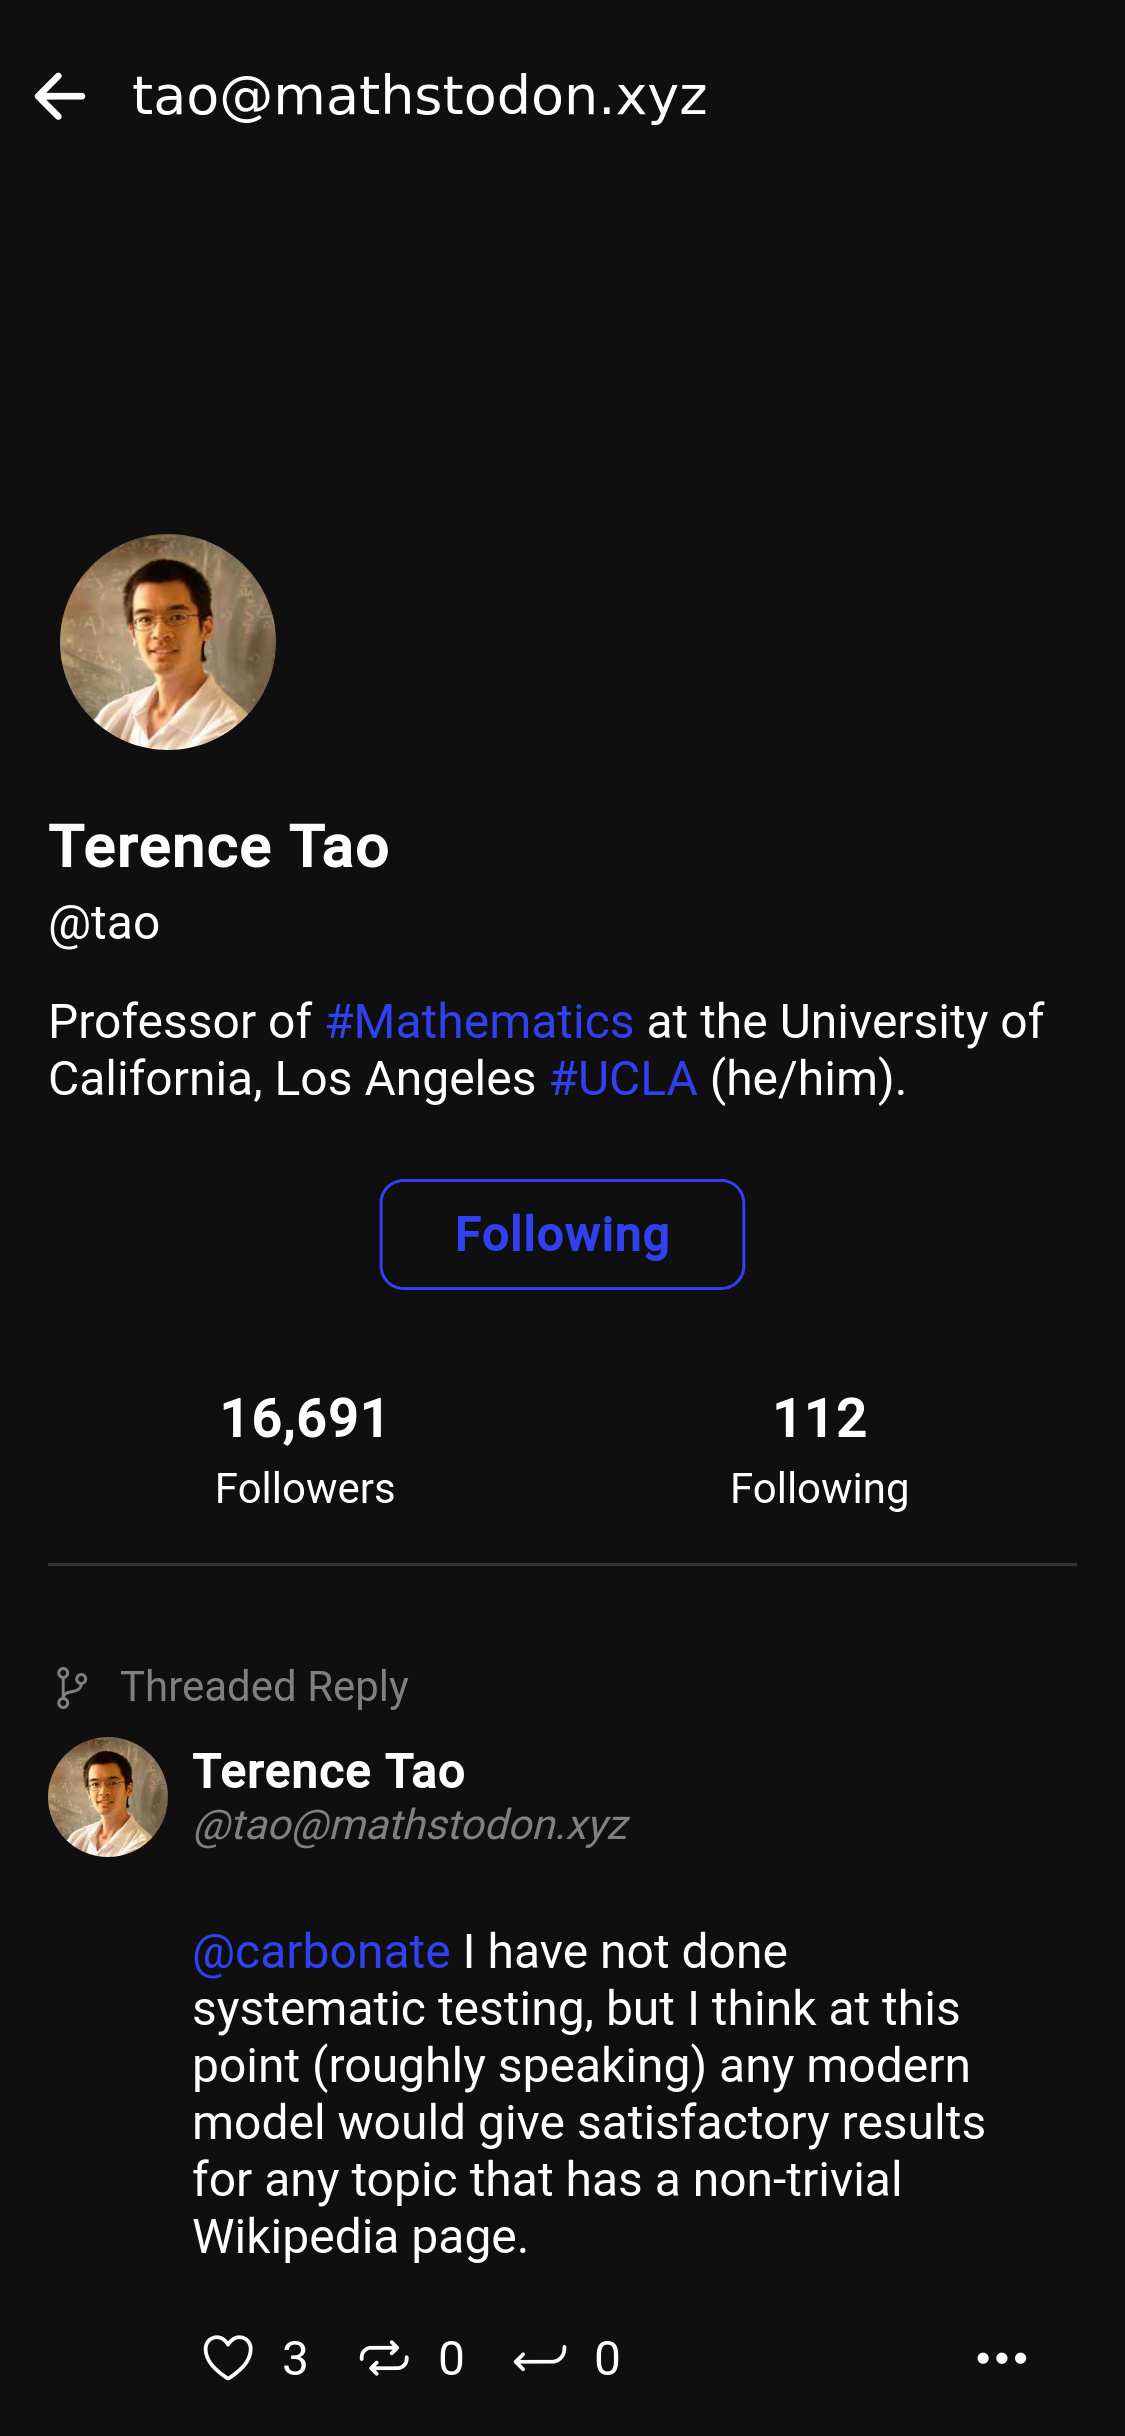
\includegraphics[width=\linewidth]{Graphics/remoteaccountprofile.png}
    \caption{Profile page of remote account}
    \label{fig:remote_profile}
  \end{minipage}
\end{figure}


\clearpage

\subsection{Remote Posts: Like, Boost, Reply}
Users can interact with remote posts in various ways, including liking, boosting (similar to retweeting), and replying. As shown in Figure~\ref{fig:like_reboost_reply}, these actions allow users to engage with posts across different instances seamlessly.

Additionally, users can view all replies to a post in a threaded format. Figure~\ref{fig:post_replies} illustrates how responses are displayed, ensuring clear and organized discussions.

\begin{figure}[htbp]
  \centering
  % First image in its own minipage
  \begin{minipage}[b]{0.45\linewidth}
    \centering
    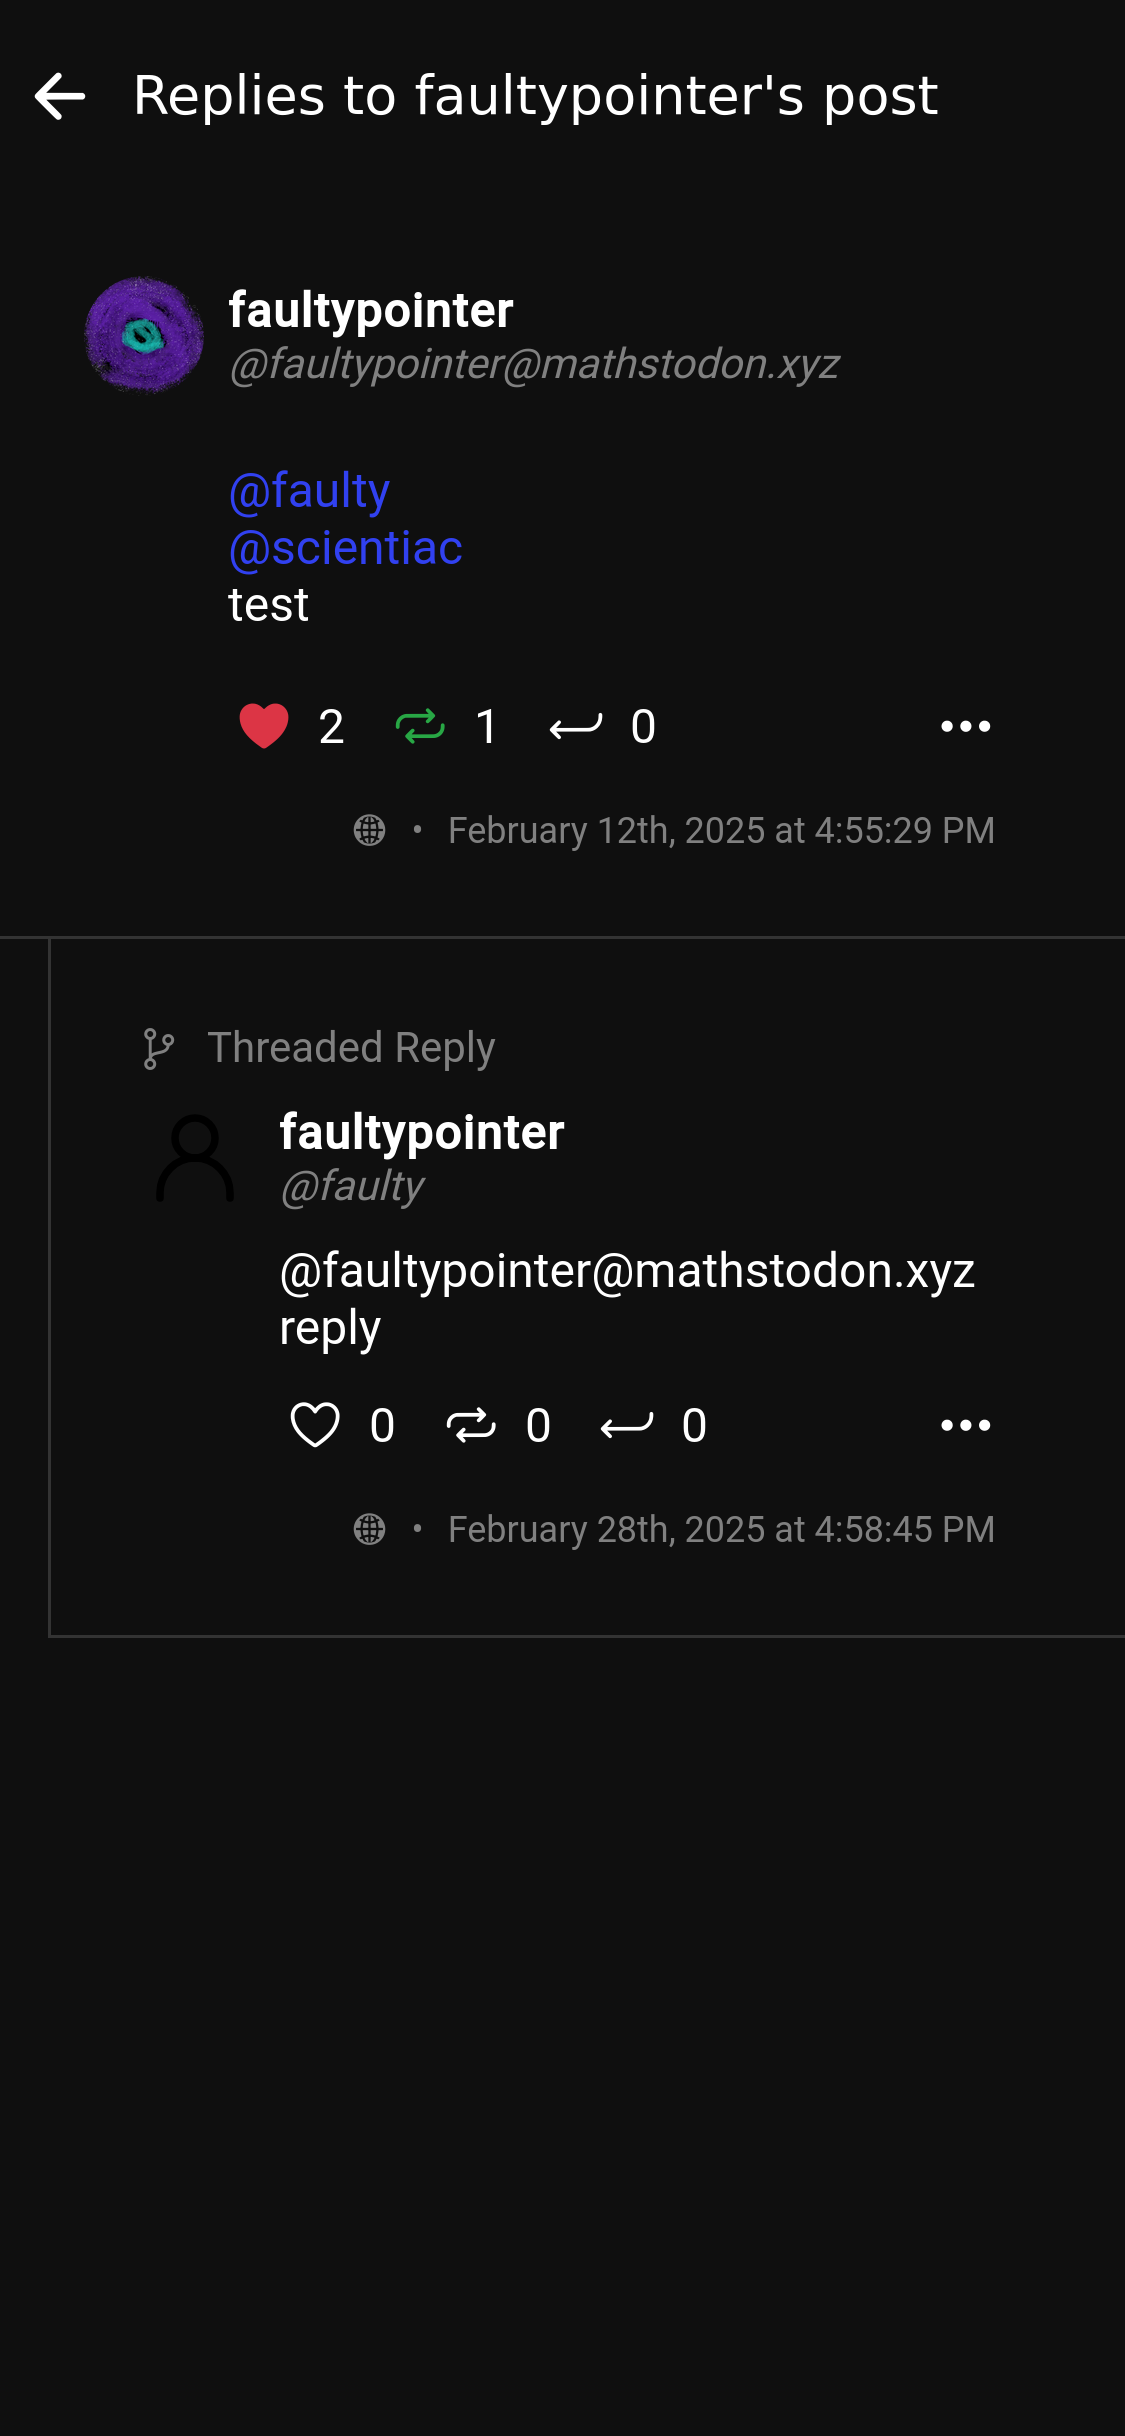
\includegraphics[width=\linewidth]{Graphics/replylikereboost.png}
    \caption{Liking, reboosting and replying to a post}
    \label{fig:like_reboost_reply}
  \end{minipage}
  \hfill % adds some space between images
  % Second image in its own minipage
  \begin{minipage}[b]{0.45\linewidth}
    \centering
    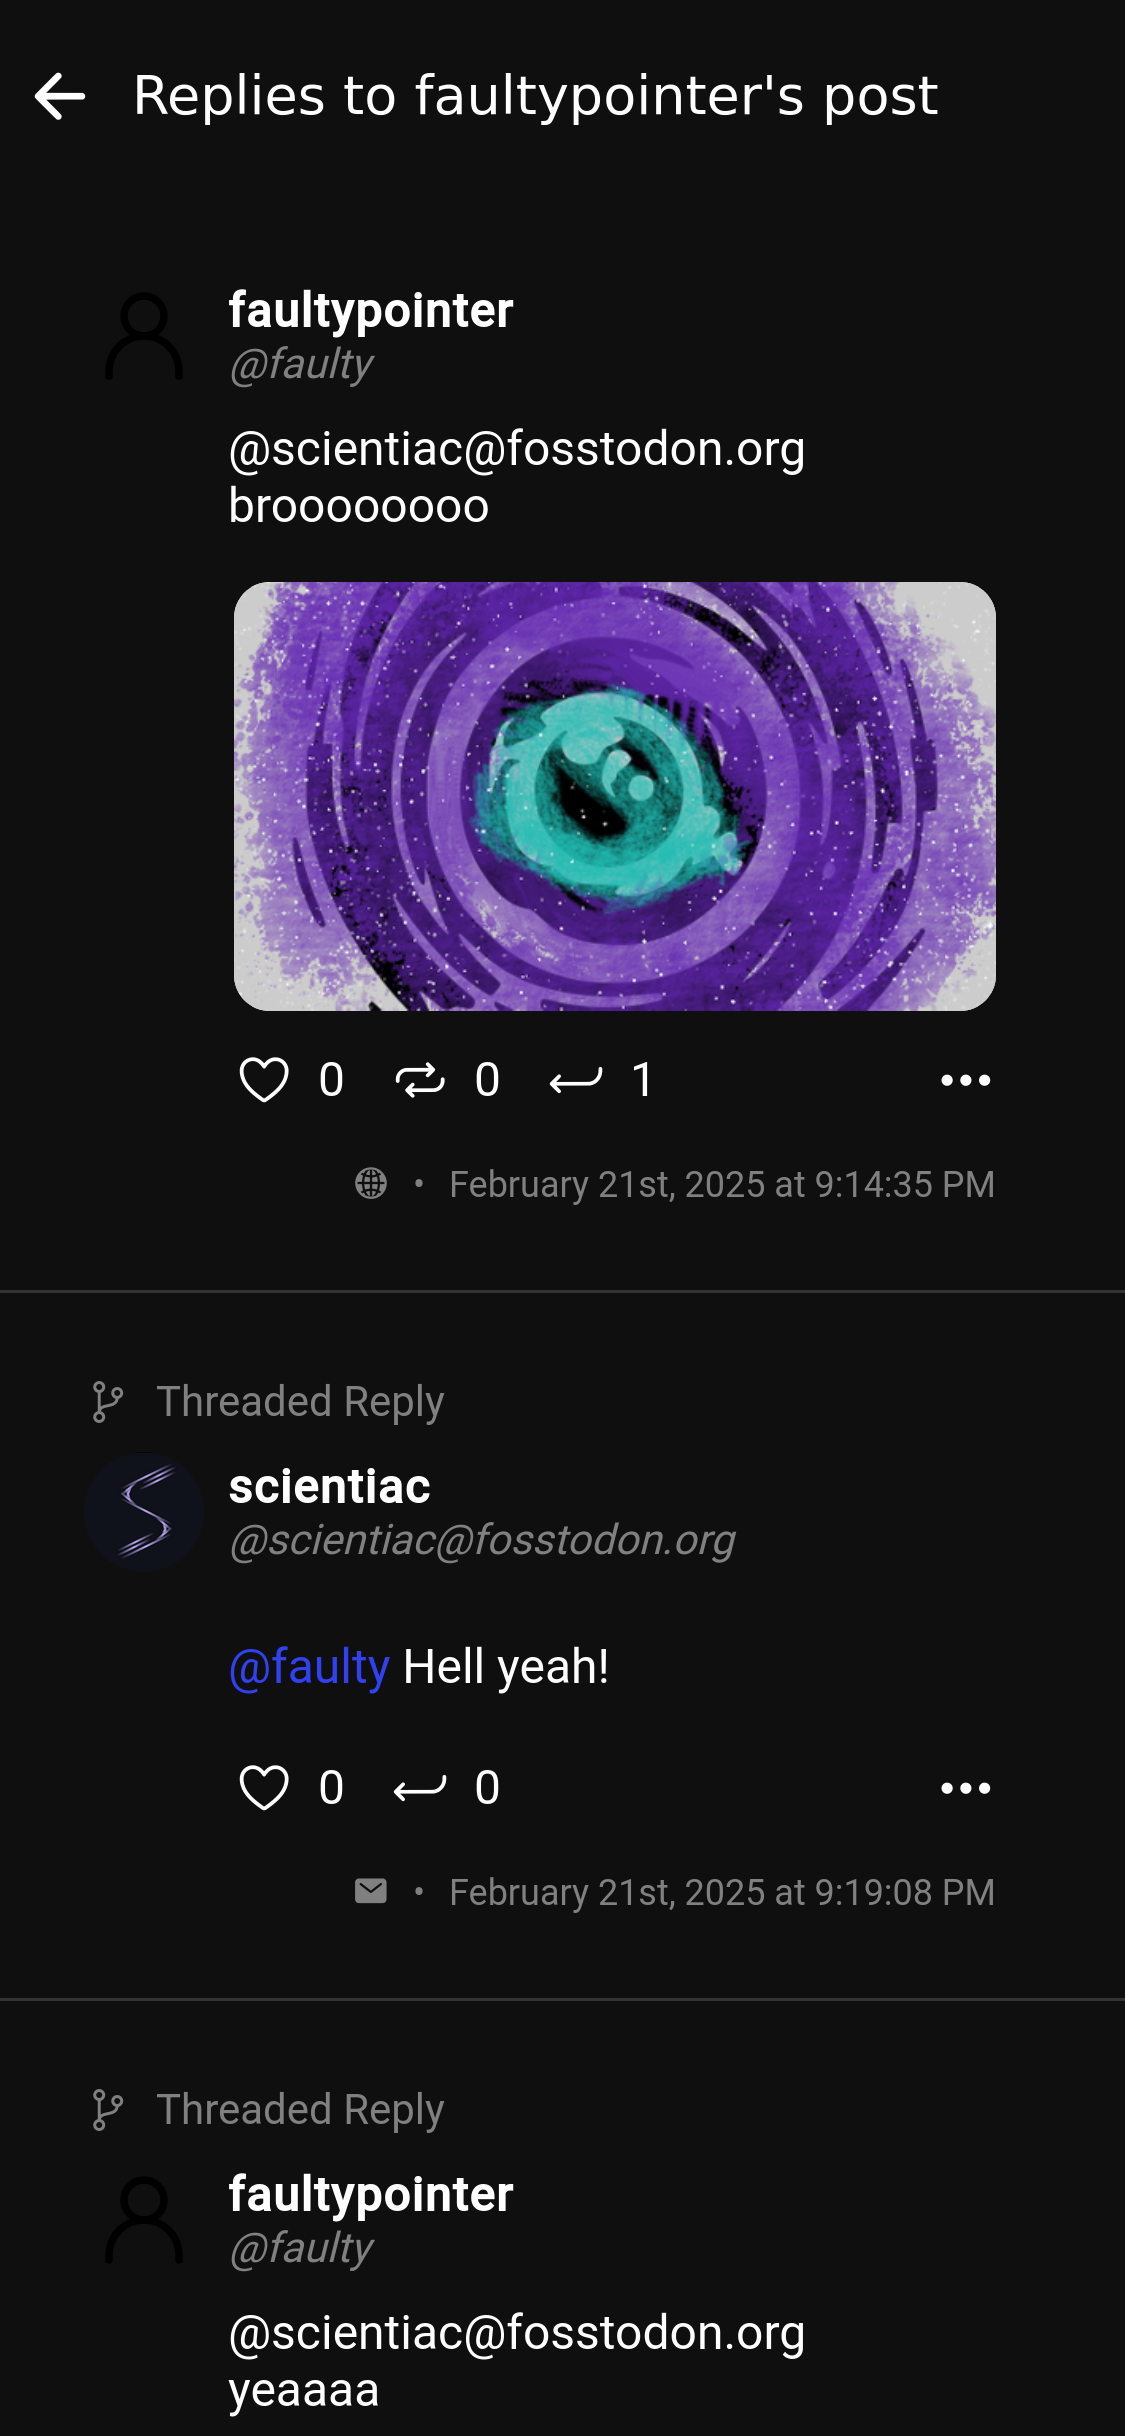
\includegraphics[width=\linewidth]{Graphics/postreplies.png}
    \caption{Viewing all the replies to a post}
    \label{fig:post_replies}
  \end{minipage}
\end{figure}

\section{More: Notifications, Followers and Following}
Users can keep track of their interactions through notifications, as shown in Figure~\ref{fig:notifications}, which provides updates on likes, replies, and follows.

Additionally, users can manage their connections through the Following and Followers list (Figure~\ref{fig:following_list}), where they can see the accounts they are following and those who follow them.

\begin{figure}[htbp]
  \centering
  % First image in its own minipage
  \begin{minipage}[b]{0.45\linewidth}
    \centering
    \includegraphics[width=\linewidth]{Graphics/Notifications.png}
    \caption{Notifications of an account}
    \label{fig:notifications}
  \end{minipage}
  \hfill % adds some space between images
  % Second image in its own minipage
  \begin{minipage}[b]{0.45\linewidth}
    \centering
    
\includegraphics[width=\linewidth]{Graphics/followerandfollowing.png}
    \caption{Following list}
    \label{fig:following_list}
  \end{minipage}
\end{figure}

